
\chapter{Florestas Aleatórias}

\begin{citacao}
	``Todos os modelos estão errados, mas alguns são úteis.''  - George Box
\end{citacao}

\section{Noções de Aprendizado de Máquina Supervisionado}

A unidade mais simples de uma Floresta Aleatória é uma Árvore de Decisão \cite{breiman2017classification} então a exposição daí partirá. Vamos construir uma árvore de decisão, mas antes precisamos de algumas definições e campo limpo. 

Em Aprendizado de Máquina Supervisionado se entende que uma \textbf{observação} é um par de um vetor $x \in \R^k$, em que cada dimensão representa uma variável mensurada e um escalar $y$ que chamaremos de \textbf{variável resposta}. Variáveis binárias podem ser representadas por pares $0$ e $1$, então usar "apenas" números reais não é uma grande limitação. Definimos o \textbf{Espaço de Mensuração} $\mathcal{X}$ como sendo o conjunto de todos os vetores $x$ possíveis para os suportes definidos e $\mathcal{Y}$ o \textbf{Espaço de Resposta}. Por exemplo: se uma dimensão deste espaço representa idade, entendemos que seu suporte está nos inteiros positivos entre $0$ e, digamos, $120$. Se uma variável é uma categoria binária, então seu suporte está em $0$ e $1$. 

As observações podem ser entendidas como pertencendo a \textbf{classes} (por exemplo, bicicletas de corrida, bicicletas de passeio, bicicletas dobráveis, etc), estando a cargo do modelador definir exatamente quais classes são essas. Um \textbf{modelo} é uma função $f: \mathcal{X} \to \mathcal{Y}$. Se $\mathcal{Y}$ é enumerável dizemos que é um modelo de \textbf{Classificação}, se for um subconjunto da reta real dizemos que é de \textbf{Regressão}. Um caso intermediário seria o de \textbf{Risco} em que $\Y = [0, \,1]$. Classificar um paciente como sendo portador de uma doença ou não é claramente um problema de classificação. Estimar o preço de um imóvel com base em suas características é um problema de regressão. 

Estimar uma Floresta Aleatória (ou Árvore de Decisão, modelo de regressão linear, o que quer que seja) é  escolher entre as inúmeras possibilidades de modelos o mais apropriado para os \textbf{dados}. Os procedimentos estatísticos que empregamos para encontrar alguma aproximação do "melhor" modelo, e podemos definir isso com uma variedade de métricas, são variados.

Algumas propriedades interessantes de um modelo, como por exemplo $\frac{\partial f}{\partial x}, \, x \in \mathcal{X}$, são trivialmente obtidas em modelos de regressão linear. Basta diferenciar um polinômio. Essa propriedade não vale em funções não-analíticas, como veremos que uma Floresta Aleatória é. Efeitos parciais são centrais para várias aplicações de econometria e demandam uma maneira de aproxima-los em outras classes, potencialmente mais interessantes que os lineares, de modelos. Ao longo deste capítulo iremos construir uma Floresta Aleatória.

\section{Construindo uma Árvore de Decisão}

Vamos estabelecer alguns fatos básicos de Teoria dos Grafos, caracterizar árvores nesse contexto e oferecer um resultado com duas condições razoavelmente fracas e suficientes para estabelecer que um grafo é uma árvore. Esse resultado tem implicações diretas em como estruturamos uma árvore de decisão, implicações estas que nos levam a estender nossa noção de grafo árvore para uma função que relaciona um espaço de mensuração $\X$ e um de resposta $\Y$.

\begin{defi}
Um \textbf{grafo} é um par $G = (V, E)$, onde $V$ é um conjunto de elementos que chamamos de \textbf{vértices} e os de $E$, \textbf{arestas}. Se uma aresta conecta dois vértices, dizemos que é aresta incidente aos vértices. Notamos o conjunto de vértices incidentes a uma aresta $h$ pela função $\phi(h)$. O número de arestas que se liga a um vértice $v$ é chamado de seu \textbf{grau}.
\end{defi}

\begin{defi}
Um \textbf{passeio} é qualquer sequência de arestas $(h_1, h_2, ..., h_{n-1})$ para os quais há uma sequência de vértices $(v_1, v_2, ..., v_n)$ de forma que $\phi(h_i) = \{v_i, v_{i+1}\}$. Uma \textbf{trilha} é um passeio em que toda aresta é distinta. Um \textbf{caminho} é uma trilha em que todo vértice é distinto. Um \textbf{ciclo} é qualquer trilha que comece e termine no mesmo vértice. Um grafo que não admite ciclos é dito \textbf{acíclico}.
\end{defi}

\begin{defi}
Um grafo $G$ é dito \textbf{conexo} se para qualquer par de vértices $x, y \in V \subset G$ há pelo menos um caminho cujo vértice inicial é $x$ e o terminal é $y$. Um subconjunto de vértices de um grafo desconexo em que vale esta propriedade é dito um \textbf{componente}.
\end{defi}


\begin{defi}
Um grafo $G$ é dito uma \textbf{árvore} se para quaisquer dois vértices de $G$ existe um caminho único os ligando. Podemos escolher um vértice arbitrário e defini-lo como a \textbf{raiz} da árvore. Os vértices que não são a raiz e têm grau unitário são ditos \textbf{folhas}. Os com grau maior que $1$ que não são a raiz são chamados \textbf{nodos}. Um conjunto disjunto de árvores é dito uma \textbf{floresta}.
\end{defi}

Se for de interesse modelar não só como certas variáveis explicativas se relacionam quantitativamente com um fenômeno, mas mais ainda a interação entre essas variáveis, existem algumas abordagens. Uma delas consistente em compor perguntas sobre os dados e para cada combinação possível de respostas atribuir alguma regra de previsão/classificação. Se as perguntas forem informativas - definiremos essa noção matematicamente mais à frente - então entende-se que grupos com respostas iguais terão resultados similares na variável explicativa, pelo menos em comparação com outros grupos. 

Perguntar perguntas sucessivamente sugere uma série de bifurcações partindo de um ponto inicial. Exatamente o que é um grafo árvore. A figura \ref{fig:arvore} ilustra uma árvore de decisão, já enriquecida com testes e regras de previsão/classificação. 

Árvores podem ser caracterizadas por duas propriedades, são conexas e acíclicas. Conexidade é importante porque garante que toda observação nova apresentada à árvore terá uma previsão garantida - afinal há sempre um caminho entre a raiz da árvore e uma folha, cada caminho representando uma regra de previsão/classificação.

A ausência de ciclos impõe que todo teste lógico que associaremos seja \textit{completo} no sentido de que toda observação pode ser avaliada e terá alguma resposta. Alguns exemplos de testes lógicos completos são: uma pessoa tem mais que $a$ cm de altura, um avião tem mais de $b$ metros de comprimento, uma pessoa ganha mais de $c$ reais por mês, o estado de nascimento de alguém é ou não o RJ, etc. Testes completos não "misturam" regras de previsão/classificação. Assim ao computar a previsão de uma observação dada, existe apenas uma regra a ser usada. Se existisse mais de uma regra de previsão para uma mesma observação então o grafo formaria ciclos. 

\begin{teo}
$G$ é uma árvore se, e somente se, é conexo e acíclico.
\end{teo}

\begin{prova}

Seja $G$ uma árvore. $G$ é trivialmente conexo pois por definição existe um caminho entre qualquer par de vértices. Suponha por absurdo que $G$ admita um ciclo. Então existe uma trilha começando e terminando em um vértice $v$ de $G$. Escolha um vértice qualquer $u$ desse ciclo. Então existe um caminho $v \to u $ e uma trilha (possivelmente um caminho) $u \to v$. Dois casos ocorrem:

\begin{itemize}
    \item Se $u \to v$ é uma trilha, então podemos entende-la como a união de dois caminhos $u \to w$ e $w \to v$. Note que nesse caso podemos truncar o caminho $v \to u$ em $w$ e estabelecemos dois caminhos distintos entre $v$ e $w$. Em contradição com $G$ ser uma árvore.

    \item Se $u \to v$ é um caminho então a contradição é imediata pois existiriam dois caminhos entre $u$ e $v$.
\end{itemize}


Agora a volta. Tome $G$ conexo e acíclico, escolha dois vértices $v$ e $u$. Suponha por absurdo que exista mais de um caminho entre $v$ e $u$. Então necessariamente existe ciclo no grafo $G$, basta "ir" por um caminho e "voltar" por outro. $G$ é uma árvore.
$\blacksquare$
\end{prova}

%Uma propriedade interessante de árvores, e que ilustra como testes seguidos são excludentes entre sim, é: 

%\begin{teo}
%Seja $G$ uma árvore. Para qualquer par de vértices $u$, $v$ existe uma aresta $h$ tal que $G - \{h\}$ é igual à união de dois grafos disjuntos $G_1$ e  $G_2$,  $u \in G_1$ e $v \in G_2$.
%\end{teo}

%\begin{prova}
%Seja $G$ uma árvore, escolha dois vértices $v \neq u$ com um caminho os ligando que passa por $h$. Suponha por absurdo que $G - \{h\}$ é conexo. Então existiam pelo menos dois caminhos entre $v$ e $u$. Se existiam dois caminhos distintos o grafo $G$ não era uma árvore. 
%\end{prova}

Vamos agora contextualizar algumas dessas definições e resultados em uma aplicação típica.

\begin{exemplo}[Classificação Binária]
 A unidade de email marketing de uma grande empresa de e-commerce quer segmentar clientes entre entusiastas de tecnologia, que engajarão felizmente com campanhas de aparelhos novos, e usuários relutantes de tecnologia, que não precisam receber esse contato nas suas caixa de email. Uma equipe selecionou algumas centenas de clientes aleatoriamente e manualmente os classificou usando entrevistas e análise de histórico de compras, um processo caro, demorado e de profundidade. Cabe agora a um analista tentar reproduzir os esforços manuais e não-escaláveis da equipe em um modelo preditivo que pode ser aplicado na base verdadeira de clientes usando os resultados do estudo.

O analista consultou o banco de dados da empresa e montou uma amostra contendo os seguintes dados: idade do cliente, percentual das compras em eletrônicos, valor médio da compra. Estamos falando de um espaço de mensuração $\X \subset \R^3$. Como a variável resposta é binária, $\Y = \{0, 1\}$. 

Um procedimento possível seria primeiro estimar por mínimos quadrados generalizados um modelo para probabilidade uma observação pertencer à uma classe $f: \R^3 \to [0, \, 1]$ e depois alguma maneira de traduzir uma probabilidade presumida pelo modelo à uma classe $g: [0, \, 1] \to \{0, 1\}$. O modelo final, neste caso, seria a composição $g \circ f: \R^3 \to \{0, 1\} $.

Modelos têm hipóteses. Nesse caso uma delas é que as variáveis explicativas são independentes, no sentido de que sua distribuição conjunta é apenas o produto de suas distribuições marginais. A intuição do analista diz que, na verdade, há sim interações entre renda e idade por exemplo. Um público mais velho que faz grandes compras em eletrônicos provavelmente é tão entusiasta quanto estudantes universitários que compram quase exclusivamente eletrônicos. O analista então pode seguir por outro caminho e enumerar uma série de perguntas sobre cada observação antes de emitir um julgamento:

\begin{itemize}
    \item O cliente tem menos de 30 anos?
    \item Mais de um quarto das compras desse cliente foram em eletrônicos?
    \item A compra média desse cliente é maior que 250 reais?
\end{itemize}

Cada pergunta aqui pode ser lida como uma função. 'O cliente tem menos de $k$ anos de idade?' é, computacionalmente,  $f: \R^2_+ \to \{0, 1\}$. Algumas perguntas são mais informativas que outras. Afinal, um usuário teve mais de 90\% das compras em eletrônicos é quase certamente um entusiasta de tecnologia, enquanto saber que um usuário tem mais de 20 anos provavelmente não é tão informativo. 

Ao compor perguntas sucessivamente chegamos em uma espécie de fluxograma de decisão. Uma boa previsão de perfil para um clientes com menos de 30 anos que comprou eletrônicos em 60\% das compras passadas e gastou 40\% a mais que a média por compra provavelmente é um usuário ávido de tecnologia. Ao passo que um usuário de 72 anos que teve 10\% das compras em eletrônicos e faz compras 40\% menores que a média provavelmente é um usuário relutante. Note que muito provavelmente um usuário de 72 anos que comprou apenas eletrônicos na plataforma é entusiasta. A composição das repostas é importante.

Note que cada vértice pode ser associado à uma pergunta única. De fato, o processo de estimação de uma árvore é o de selecionar quais perguntas são feitas com quais parâmetros em quais vértices. 
\end{exemplo}

O ponto importante é que podemos traduzir um grafo árvore $G$ em um modelo, basta associar a cada nodo alguma função representando um teste lógico sobre uma observação $x \in \X$, para cada folha uma previsão $y \in \Y$ e uma raiz. Com isso queremos dizer que para todo nodo $n_i \in G$ existe um teste $\tau_{n_i}(x) : X \subset \X \to [0, 1]$ e que existe uma raiz $v$, que será o primeiro teste a ser respondido. Por construção, para cada observação $x \in \X$ existe um único caminho com os nodos $ \{n_i \, | \, \tau_{n_i}(x) = 1\}$ e portanto uma única previsão $y \in \Y$. 


\begin{figure}
    \centering
    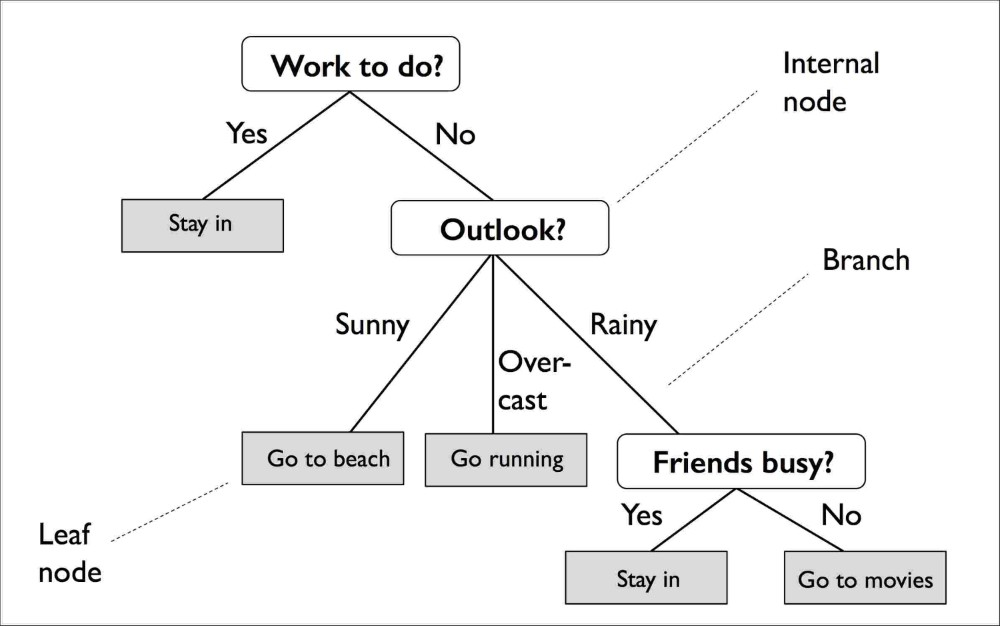
\includegraphics[scale = .55]{imagens/arvore.png}
    \caption{Um exemplo de árvore de decisão. Elaboração própria.}
    \label{fig:arvore}
\end{figure}


\begin{defi}
Seja $\X, \Y$ um par de espaços de mensuração e resposta. Uma \textbf{Árvore de Decisão} é uma função $\A: \X \to \Y$, onde $\Y$ é enumerável, associada à uma árvore $G$. Se $\Y$ for um subconjunto convexo da reta então chamamos de \textbf{Árvore de Regressão}.
\end{defi}

\begin{exemplo}[Regressão]
 Uma empresa de tecnologia no ramo de venda e aluguel de imóveis quer trabalhar em um modelo de precificação de aluguel. A ideia é que donos de imóveis recebam um valor sugerido compatível com o mercado e embutir isso no serviço.
 
 Um analista coletou dados de aluguel e algumas informações básicas do apartamento. Área, número de quartos, de banheiros, se aceita animais, se é mobiliado e em qual cidade está localizado. A média de cada variável, por cidade, é:
 
 
\begin{tabular}{l|r|r|r|r|r|r|r|r}
\hline
cidade & area & quartos & banheiros & vagas & andar & mobiliado & aluguel & aceita\_animal\\
\hline
Belo Horizonte & 136.71745 & 2.863596 & 2.167405 & 1.7245350 & 3.514615 & 0.1302037 & 2765.900 & 0.7307352\\
\hline
Porto Alegre & 93.27658 & 2.086430 & 1.652550 & 0.9749352 & 3.949006 & 0.2644771 & 2069.884 & 0.8461538\\
\hline
Rio de Janeiro & 93.14216 & 2.158964 & 1.657563 & 0.6792717 & 5.247899 & 0.2626050 & 2774.703 & 0.8011204\\
\hline
São Paulo & 124.69289 & 2.395466 & 2.204030 & 1.6002713 & 5.608216 & 0.2600271 & 3600.296 & 0.7512110\\
\hline
\end{tabular}

 
 E a árvore de regressão estimada foi:
 
 \begin{figure}
    \centering
    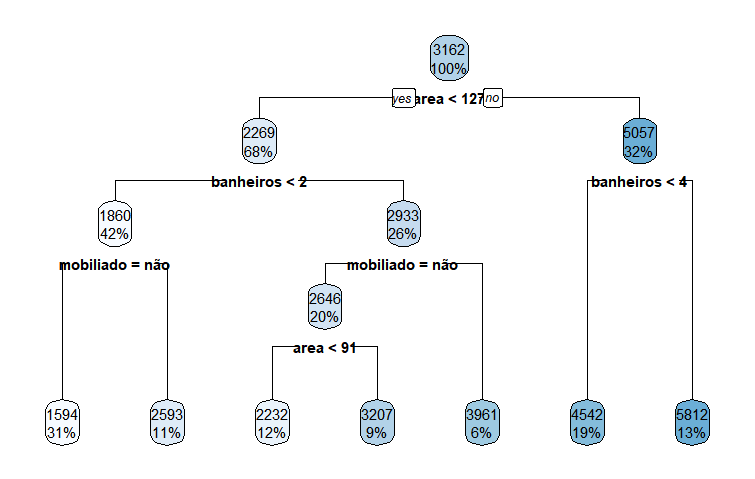
\includegraphics[scale = .55]{imagens/arvore_decisao_houses.png}
    \caption{Um exemplo de árvore de regressão. Elaboração própria.}
    \label{fig:arvore_reg}
\end{figure}
 
 Os valores abaixo das folhas são as previsões. 


 
 
\end{exemplo}





\section{Noções de Estimação de uma Árvore de Decisão}

Como podemos traduzir uma amostra $A$ em uma árvore de decisão $\A$? Uma abordagem candidata é o procedimento original apresentado na primeira edição de \citeonline{breiman2017classification}.

Imagine que temos uma massa de dados, uma nuvem de pontos em algum espaço de mensuração. 

REESCREVER A PARTIR DAQUI

%Primeiro definimos a \textbf{proporção} de um vértice como um vetor contendo a proporção de cada classe observada nos dados que chegaram ao vértice. Depois, a \textbf{Impureza} do nodo. A função $\I(\cdot)$ mapeia um nodo em um número positivo limitado superiormente por um real $I$ de forma que a impureza de um nodo cuja proporção seja igual para todas as classes seja $0$ e a impureza de um nodo cuja proporção seja unitária para alguma classe seja $I$. Precisamos impor apenas que $\I(\cdot)$ seja monotonamente crescente em relação à probabilidade de cada classe. O valor específico da impureza não é relevante, desde que aumente monotonamente em relação à heterogeneidade de proporções observadas.

%Tome uma divisão $D_i$ qualquer. Ela rende duas subamostras/divisões que podem ou não serem terminais, $D_{iA}$ e $D_{iB}$. Defina $P_A (D_i)$ como a proporção de casos que chegam em $D_i$ e vão para $D_{iA}$ e o mesmo para $P_B (D_i)$. A \textbf{Qualidade} da divisão é dada pela variação na impureza: $\mathcal{Q} (D_i) := \I(D_i) - P_A(D_i) \I (D_{iA}) - P_B(D_i) \I (D_{iB})$.


%Note que a qualidade é uma variável aleatória. O processo de formar uma árvore de decisão a partir de um certo conjunto de dados é chamado de treinar a árvore. Escolher a divisão adequada envolve muitos recursos computacionais e selecionar a divisão que maximize a qualidade dentre as potenciais. Qualquer regra computável pode ser usada: um valor ser maior ou menor que um certo patamar, estar em uma certa faixa, etc. Os aspectos algorítmicos deste problema são interessantes porém fogem ao escopo desta monografia, discussões podem ser encontradas em \citeonline{de1991distance}.
 
 \section{Construindo uma Floresta Aleatória}
 
 A agregação das predições de árvores construídas a partir de pedaços diferentes da amostra é um passo seguinte e natural à modelagem anteriormente apresentada. Como os procedimentos de escolha de divisões são estocásticos, árvores individuais de decisão podem apresentar vieses ou baixa performance ao acaso. Se um número grande de árvores é agregado e não há relação sistemática do erro de predição com alguma variável preditiva, então os erros devem se anular com o aumento do número de árvores.
 
 %\begin{defi}
 %Seja $A$ uma instância de um Banco $(\mathcal{X}, \C)$. Existe um conjunto de subamostras únicas dessa instância, $B = \{ B_1, B_2, ..., B_k\}$  independentes. Treine em cada elemento de $B$ uma árvore de decisão $\A_i$ e chame de $F(x)$ o conjunto de imagens obtidas ao aplicar cada $\A_i$ a uma observação $x$ da instância $A$. Uma \textbf{Floresta Aleatória} é um classificador $\F : F(x) \to \C$. 
  %\end{defi}
  
  %\begin{defi}
 % Seja $A$ uma instância de um Banco $(\mathcal{X}, \C)$ com $n$ observações. Seja $F$ um conjunto de $k$ árvores de decisão treinadas em $A$ de acordo com a definição anterior. Seja $x_i$ a $i$-ésima observação da instância $A$ e, por fim, $\1(\cdot)$ a função indicadora. A \textbf{Margem} da floresta aleatória $\F$ formada pelas árvores de decisão $\A_j$ na observação $x_i$ é a função $M(\F, x_i) := \sum_{j=1}^k \1 ( \A_j (x_i) = \C(x_i) ) - \sum_{j=1}^k \1  ( \A_j (x_i) \neq \C(x_i) )$.
 % \end{defi}
  
 
 % \begin{defi}
 %Para uma observação $x$ de uma instância $A$, o \textbf{Erro de Generalização} $G(\F, x) := \Prob (M(\F, A, x)) < 0)$.  \end{defi}
  
 % A margem provê uma medida do quão precisa é a floresta em votar corretamente na classe verdadeira da observação. Uma margem maior sinaliza uma maior capacidade da floresta de discriminar o dado observado entre possíveis classes.  

 %\begin{teo}[Convergência do Erro de Generalização] Seja $A$ uma instância de um Banco $(\mathcal{X}, \C)$. Defina a sequência $E_k = \{ G(\F_k, A, x) \}$ de forma que $\F_k = \F_{k-1} \bigcup \A_k $,  Tome as classes possíveis $\C = \{1,2,3,...,c,...,J \}$ e uma observação $x$, tal que $\C(x) = c$. Então $E_k \to \sum_{i=1}^k \1 ( \A_i (x) = c ) - \underset{}{\text{Max}} \sum_{i=1}^k \1  ( \A_i (x) \neq c) $
 
% \end{teo}
 
Alguns refinamentos muito interessantes podem ser feitos. \textit{Bagging}, a ideia de expor árvores diferentes da floresta à observações e variáveis explicativas diferentes. \textit{Boosting}, treinar uma árvore no resíduo de outra, fazendo a floresta aprender lentamente, incorporando padrões mais sutis. 
 
 
 
 \begin{prova}
 Ver o Apêndice 1 de \citeonline{breiman2001random}. \blacksquare
 \end{prova}
